% todo: information if someone wants to make a resource compatible with GB: what kind of things it should expose
% todo: diagram include third-party for auth
% todo: avoid generic titles

\chapter{Interoperability Layer for Clinical Research Systems}

In this chapter we are presenting the solution for the first objective of the project:
setting up an interoperability layer for the main open-source clinical research systems, namely tranSMART, i2b2 and their respective derivations.
The general design of the solution is first presented, then the steps that are required to implement this system are explained.

\section{Design of the Interoperability Layer}
% todo: here give the big picture
% todo: give a roadmap
% todo: integrate running exmaple? the query below works well?

This section describes in details the design of the solution chosen chapter~\ref{sec:sysdesign}. 
It aims to allow the cohort explorer UI Glowing Bear to support the following systems:
\begin{itemize}
    \item i2b2
    \item SHRINE 
    \item tranSMART 17.1 (REST API v2)
    \item tranSMART 16.2 (REST API v1)
\end{itemize}

Because of the fundamental differences in the APIs, it is not possible to browse at the same time. 
After being logged in, the user is able to choose from which resource do the queries.
A resource is defined as an instance of one the supported systems.

Figure~\ref{fig:sysdiagramobj1} shows the system diagram after completion of the objective 1.
We can see that IRCT acts as a back end component for Glowing Bear, all its communications go through it using the PIC-SURE API.

\begin{figure}[h!]
    \centering
    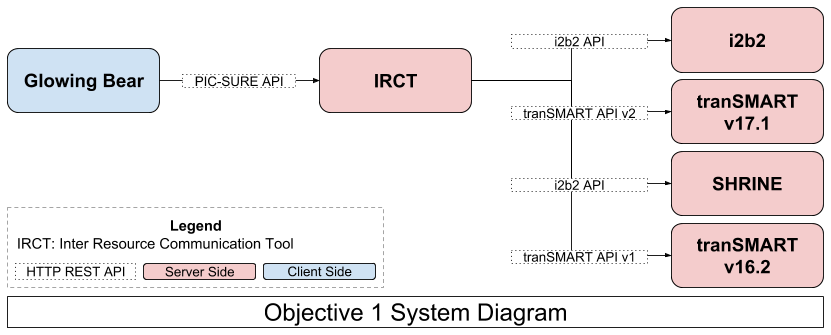
\includegraphics[width=1\textwidth]{figures/sys_diagram_obj1.png}
    \caption{System diagram of objective 1: Interoperability layer for a common front end for clinical research platforms.}
    \label{fig:sysdiagramobj1}
\end{figure}

todo: say that it wont query all the resources at once: some may support soem things or not 



\paragraph{Interoperability Layer}

\paragraph{Connectors}
what is supported for each connector
GB enable disable stuff

\paragraph{Authentication \& Authorization}
TBD: the authentication \& authorization still needs to be decided.

%The authentication and authorization is delegated to a third-party using the OpenID Connect protocol~\cite{openidconnect}.

\subsection{Glowing Bear API calls}

One of the main implementation challenge is replacing in Glowing Bear the tranSMART API v2 by the PIC-SURE API.
In Glowing Bear, all the operations the user undertakes have the objective of constructing a query to select data.
In order to give an overview of the goal of the changes in Glowing Bear, see below an example of a query with the tranSMART API v2 and its equivalent using the PIC-SURE API.
The query exports the age and gender for all patients aged from 20 to 25 years old in the \emph{CATEGORICAL\_VALUES} study.

% todo: transmart has an export field (with and all), does pic-sure really returns directly the full resp?

\paragraph{tranSMART API v2 Example Query}
\begin{verbatim}
POST /export/<id>/run

{ "constraint": {
"type": "and",
"args": [
  {
    "type": "and",
    "args": [ {
        "type": "subselection", "dimension": "patient",
        "constraint": {
          "type": "and",
          "args": [
            {
              "type": "and",
              "args": [
                { "type": "concept", "conceptCode": "CV:DEM:AGE" },
                { "type": "value", "valueType": "NUMERIC", "operator": ">=", "value": 20 },
                { "type": "value", "valueType": "NUMERIC", "operator": "<=", "value": 25 }
              ]
            },
            { "type": "study_name", "studyId": "CATEGORICAL_VALUES" }
          ]
        } } ]
  }, {
    "type": "or",
    "args": [
      {
        "type": "and",
        "args": [
          { "type": "concept", "conceptCode": "CV:DEM:AGE" },
          { "type": "study_name", "studyId": "CATEGORICAL_VALUES" }
        ]
      }, {
        "type": "and",
        "args": [
          { "type": "concept", "conceptCode": "CV:DEM:SEX:F" },
          { "type": "study_name", "studyId": "CATEGORICAL_VALUES" }
        ]
      }, {
        "type": "and",
        "args": [
          { "type": "concept", "conceptCode": "CV:DEM:SEX:M" },
          { "type": "study_name", "studyId": "CATEGORICAL_VALUES" }
        ]
      } ]
  }
]
},
"elements": 
    [{ "dataType": "clinical", "format": "TSV", "dataView": "default" }]
}
\end{verbatim}

\paragraph{PIC-SURE API Equivalent Query}
\begin{verbatim}
POST /rest/queryService/runQuery?full_response
{
  "select": [ {
    "field": {
        "pui": "/<resource>/Public Studies/CATEGORICAL_VALUES/Demography/Age/",
        "dataType": "INTEGER"
    }
  }, {
    "field": {
        "pui": "/<resource>/Public Studies/CATEGORICAL_VALUES/Demography/Gender/Male/",
        "dataType": "ENUM_VALUE"
    }
  }, {
    "field": {
        "pui": "/<resource>/Public Studies/CATEGORICAL_VALUES/Demography/Gender/Female/",
        "dataType": "ENUM_VALUE"
    }
  } ],
  "where": [
        {
            "field": {
                "pui": "/<resource>/Public Studies/CATEGORICAL_VALUES/Demography/Age/",
                "dataType": "INTEGER"
            },
            "predicate": "CONSTRAIN_VALUE_NUMERIC",
            "fields": { "OPERATOR": ">=", "CONSTRAINT": "20" }
        }, {
            "field": {
                "pui": "/<resource>/Public Studies/CATEGORICAL_VALUES/Demography/Age/",
                "dataType": "INTEGER"
            },
            "predicate": "CONSTRAIN_VALUE_NUMERIC",
            "fields": { "OPERATOR": "<=", "CONSTRAINT": "25" },
            "logicalOperator": "AND"
        }, {
            "field": {
                "pui": "/<resource>/Public Studies/CATEGORICAL_VALUES/",
                "dataType": "STUDY"
            },
            "predicate": "CONTAINS",
            "logicalOperator": "AND"
        }
    ]
  "alias": "My query"
}
\end{verbatim}

